\documentclass[11pt,a4paper,openany]{report}

\title{CS6890 HW02}
\author{Jonathan Arndt }
\date{July 16 2017}

\usepackage{amsmath,mathtools}
\usepackage{systeme}
\usepackage[utf8]{inputenc}
\usepackage{newunicodechar}
\usepackage{amsmath}


%% the first is the “unknown minus” (U+2212), the second is a hyphen
\newunicodechar{−}{-}

\newenvironment{sysmatrix}[1]
 {\left(\begin{array}{@{}#1@{}}}
 {\end{array}\right)}
\newcommand{\ro}[1]{%
  \xrightarrow{\mathmakebox[\rowidth]{#1}}%
}
\newlength{\rowidth}% row operation width
\AtBeginDocument{\setlength{\rowidth}{3em}}

\begin{document}

\maketitle

\section*{Problem 1}
Transform the following LP into the standard form.

\begin{itemize}
  \item minimize \(z=2x_1-3x_2+5x_3+x_4\) subject to
  \begin{enumerate}
    \item \(-x_1+3x_2-x_3+2x_4\leq-12\)
    \item \(5x_1+x_2+4x_3-x_4\geq10\)
    \item \(3x_1-2x_2+x_3-x_4=-8\)
    \item \(x_1,x_2,x_3,x_4\geq0\)
  \end{enumerate}
\end{itemize}
Only \(\leq\) inequalitites. Multiply 2. by -1. \(-5x_1-x_2-4x_3+x_4\leq10\)\\\\
To transform a minimzation problem to a maximization problem, multiply the objective function by -1. \(z=-2x_1+3x_2-5x_3-x_4\) \\\\
Transform \(=\) inequality by turning it into two inequalitites with 3..\\  \(3x_1-2x_2+x_3-x_4\leq-8\) and \(-3x_1+2x_2-x_3+x_4\leq8\)\\\\
Becomes:
\begin{itemize}
  \item maximize \(z=-2x_1+3x_2-5x_3-x_4\) subject to
  \begin{enumerate}
    \item \(-x_1+3x_2-x_3+2x_4\leq-12\)
    \item \(-5x_1-x_2-4x_3+x_4\leq10\)
    \item \(3x_1-2x_2+x_3-x_4\leq-8\)
    \item \(-3x_1+2x_2-x_3+x_4\leq8\)
    \item \(x_1,x_2,x_3,x_4\geq0\)
  \end{enumerate}
\end{itemize}

\newpage
\section*{Problem 2}
Nick’s Furniture, LLC produces two types of wooden chairs - A and B. The manufacture of chair A requires 2 hours of assembly time and 4 hours of finishing. Chair B requires 3 hours to assemble and 3 hours to finish. The company estimates that next week 72 hours will be available for assembly operations and 108 hours for finishing. The unit profits for chairs A and B are \$10 and \$9, respectively. It is also estimated that the maximum demand for chair B will be 16. Formulate an LP model and solve it graphically to answer the question of what is the optimal product mix for the company next week.\\

Becomes:
\begin{itemize}
  \item maximize \(z=10x_1+9x_2\) subject to
  \begin{enumerate}
    \item \(2x_1+3x_2\leq72\)
    \item \(4x_1+3x_2\leq108\)
    \item \(x_1\geq0,x_2\geq16\)
  \end{enumerate}
\end{itemize}
\begin{center}
  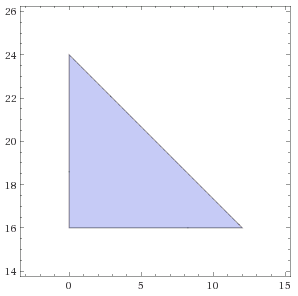
\includegraphics[height=10cm]{images/p2_1}
\end{center}
With corner points being: (0,24)=216,(0,16)=144,\((\frac{40}{3},16)\)=\(\frac{832}{3}\)$\approx$277\\\\
Thus the maximum solution is: \(x_1=\frac{40}{3},x_2=16\)

\newpage
\section*{Problem 3}
\begin{itemize}
  \item minimize \(z=4x_1+5x_2\) subject to
  \begin{enumerate}
    \item \(3x_1+2x_2\leq24\)
    \item \(x_1\geq5\)
    \item \(3x_1-x_2\leq6\)
    \item \(x_1,x_2\geq0\)
  \end{enumerate}
\end{itemize}
\begin{center}
  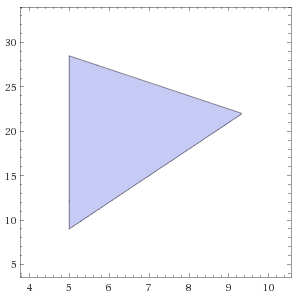
\includegraphics[height=10cm]{images/p3_1}
\end{center}
With corner points being: (5,9)=65,(4,6)=46,\((5,\frac{9}{2})\)=\(\frac{85}{2}\)=22.5\\\\
Thus the minimum solution is: \(x_1=5,x_2=\frac{9}{2}\)

\newpage
\section*{Problem 4}
\begin{itemize}
  \item minimize \(z=x_1-4x_2\) subject to
  \begin{enumerate}
    \item \(x_1+x_2\leq12\)
    \item \(-2x_1+x_2\leq4\)
    \item \(x_2\leq8\)
    \item \(x_1-3x_2\leq4\)
    \item \(x_1,x_2\geq0\)
  \end{enumerate}
\end{itemize}
\begin{center}
  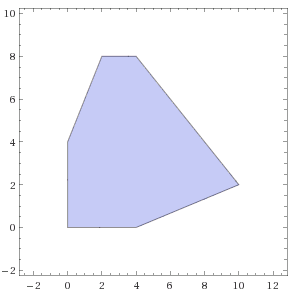
\includegraphics[height=10cm]{images/p4_1}
\end{center}
With corner points being: (0,0)=0,(4,0)=4,(0,4)=-16,(2,8)=-30,(4,8)=-28,(10,2)=2\\\\
Thus the minimum solution is: \(x_1=2,x_2=8\)

\newpage
\section*{Problem 5}
\begin{itemize}
  \item maximize \(z=6x_1+8x_2\) subject to
  \begin{enumerate}
    \item \(x_1+4x_2\leq16\)
    \item \(3x_1+4x_2\leq24\)
    \item \(3x_1-4x_2\leq12\)
    \item \(x_1,x_2\geq0\)
  \end{enumerate}
\end{itemize}
\begin{center}
  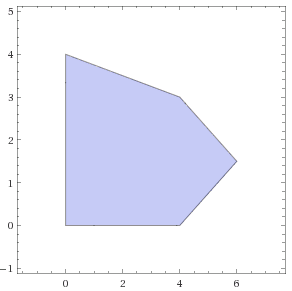
\includegraphics[height=10cm]{images/p5_1}
\end{center}
With corner points being: (0,0)=0,(0,4)=32,(4,0)=24,(4,3)=48,(6,\(\frac{1}{2}\))=40\\\\
Thus the maximize solution is: \(x_1=4,x_2=3\)

\newpage
\section*{Problem 6}
\begin{itemize}
  \item maximize \(z=x_1+2x_2\) subject to
  \begin{enumerate}
    \item \(-2x_1+x_2\leq2\)
    \item \(2x_1+5x_2\geq10\)
    \item \(x_1-4x_2\leq2\)
    \item \(x_1,x_2\geq0\)
  \end{enumerate}
\end{itemize}
\begin{center}
  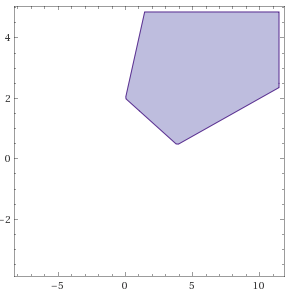
\includegraphics[height=10cm]{images/p6_1}
\end{center}
With corner points being: (0,2)=4,(\(\frac{50}{13},\frac{6}{13})=\frac{62}{13}\),\((\infty,\infty)=\infty\)\\\\
Thus the maximize solution is: \(x_1=\infty,x_2=\infty\)

\newpage
\section*{Problem 7}
Given the polyhedral set \(S = {(x1, x2)|x1 +x2 \leq 10, −x1 +x2 \leq 6, x1 −4x2 \leq 0}\).
\begin{itemize}
  \item Find all extreme points of S.
  \item Represent the point x = (2, 4) as a convex combination of the extreme points.
\end{itemize}\\\\
\(
\begin{sysmatrix}{rr|r}
  1 & 1 & 10 \\
  -1 & 1 & 6 \\
\end{sysmatrix}
\) Then \((x_1,x_2)=(2,8)\)
\\\\
\(
\begin{sysmatrix}{rr|r}
  1 & 1 & 10 \\
  1 & 4 & 0 \\
\end{sysmatrix}
\) Then \((x_1,x_2)=(8,2)\)
\\\\
\(
\begin{sysmatrix}{rr|r}
  -1 & 1 & 6 \\
  1 & 4 & 0 \\
\end{sysmatrix}
\) Then \((x_1,x_2)=(-8,-2)\)
\\\\\\\\
\((2,4)=x_1(2,8)+x_2(8,2)+x_3(-8,-2)\)
\[
\systeme*{
2x_1+8x_2-8x_3=2,
8x_1+2x_2-2x_3=4,
x_1+x_2+x_3=1
}
\]

Row reducing leads to \((x_1,x_2,x_3)=(\frac{7}{15},\frac{1}{3},\frac{1}{5})\)

The point as a convex combination of the exteme points is:

\((2,4)=\frac{7}{15}(2,8)+\frac{1}{3}(8,2)+\frac{1}{5}(-8,-2)\)

\newpage
\section*{Problem 8}
Let S1 and S2 be convex sets. Is S1 \(\cap\) S2 convex? Is S1 \(\cup\) S2 convex? You can either state your answers as proofs or, if you do not feel comfortable with proofs, justify your answers with a few sentences.\\\\

Yes for intersection and no for union.\\

No for union because imagine 2 circles (which are convex sets) union then there will exist a piece that can't connect on top of each circle.

\end{document}
